%
% bezier.tex
%
% (c) 2020 Prof Dr Andreas Müller, Hochschule Rapperswil
%

\subsection{Bézier-Kurven und Splines in der Ebene
\label{buch:subsection:bezier}}
Spline-Interpolation kann auch verwendet werden, um Kurven in der Ebene
oder im Raum zu approximieren.
In der Computergraphik ist dabei besonders wichtig, dass sich Kurvenpunkte
mit einfachen Operationen aus einer kleinen Zahl von Parametern berechnen
lassen, damit sie zum Beispiel von einem Graphikprozessor berechnet
werden können.
Dieser Abschnitt soll daher den Zusammenhang zwischen Bézier-Kurven und
Splines aufzeigen.

%
% Kurven in der Ebene
%
\subsubsection{Kurven in der Ebene}
Eine Kurve in der Ebene ist eine Abbildung
\[
\gamma \colon \mathbb R \to \mathbb R^2 : t \mapsto \gamma(t) = (x(t),y(t)),
\]
genannt die Parameterdarstellung der Kurve.
Man kann sich den Parameter $t$ als die Zeit vorstellen und die Funktionen
$x(t)$ bzw.~$y(t)$ als die Koordinaten eines sich auf der Kurve bewegenden
Punktes zur Zeit $t$.
Der Tangentialvektor
\[
\dot{\gamma}(t)
=
\frac{d\gamma(t)}{dt}
=
\begin{pmatrix}
\dot{x}(t)\\\dot{y}(t)
\end{pmatrix}
\]
kann entsprechend auch als der Geschwindigkeitsvektor zur Zeit $t$ 
intepretiert werden.

\begin{beispiel}
Ein Kreis in der Ebene kann beschreiben weren mit der Parameterisierung
\[
\gamma(t) = (\cos t, \sin t)
\qquad
\text{mit Geschwindigkeitsvektor}
\qquad
\dot{\gamma}(t)
=
\begin{pmatrix}
-\sin t\\\cos t
\end{pmatrix}.
\]
Der Betrag der Geschwindigkeit ist $|\dot{\gamma}(t)|^2=\sin^2t+\cos^2t=1$,
also konstant.
\end{beispiel}

\begin{beispiel}
Jeder Graph einer Funktion $f(x)$ kann als Kurve mit der Parameterisierung
\[
\gamma \colon \mathbb R\to\mathbb R^2 : t \mapsto (t, f(t))
\]
aufgefasst werden.
Der Tangentialvektor ist
\[
\dot{\gamma}(t)
=
\begin{pmatrix}
1\\f'(t)
\end{pmatrix}.
\]
Insbesondere ist die Geschwindigkeit $|\dot{\gamma}(t)|^2=1+f'(x)^2|>1$
im Allgemeinen nicht konstant.
\end{beispiel}

Das Beispiel zeigt, dass Graphen von Funktionen zwar als Kurven aufgefasst
werden können, als Bahnbeschreibung zum Beispiel für einen Roboter taugen
sie dagegen kaum.
Andererseits haben die Spline-Interpolationsfunktionen die schöne
Eigenschaft, dass die mittlere zweite Ableitung minimiert wird.
Sie sind daher ``die am wenigsten gekrümmten'' Kurven, die durch die
Stützstellen gehen. 
Eine solche Minimaleigenschaft für die Bahnkurve eines Roboters könnte eine
Bahn beschreiben, die sich mit maximaler Geschwindigkeit durchfahren lässt.
Die Zentripetalkraft, die die Räder in den Kurven aufbringen müssen,
kann nicht grösser sein als die Haftreibung.
Je grösser die Bahnkrümmung, desto grösser auch die Zentripetalkraft und
desto langsamer muss der Roboter durch die Kurve fahren, um nicht ins
Rutschen zu geraten.

Wir betrachten also eine Kurve, die durch die vorgegebene Punkte
\[
P_0 = (x_0, y_0),\;
P_1 = (x_1, y_1), \;
P_2 = (x_2, y_2),
\dots,
P_n=(x_n, y_n)
\]
gehen soll.
Wir fordern, dass der Punkt $P_i$ zum Zeitpunkt $t_i$ durchlaufen wird.
Wir entfernen uns hier etwas von der Anwendung einer Robotersteuerung,
da würde man nur die Punkte vorgeben und dann eine Bahn suchen, mit der
sich die Zeitpunkte $t_i$ so wählen lassen, dass die Gesamtzeit minimal
wird.
Die Funktionen $x(t)$ und $y(t)$ erfüllen jetzt also
\[
x(t_i) = x_i
\qquad\text{und}\qquad
y(t_i) = y_i.
\]
Das Problem, eine ebene Kurve durch die Punkte $P_i$ zu parametrisieren
ist damit zerlegt worden in zwei unabhängige Interolationsprobleme
für die Funktionen $x(t)$ und $y(t)$.

Jedes in diesem Kapitel besprochene Interpolationsverfahren kann dafür
eine mögliche Lösung liefern, wobei sich die Spline-Interpolation wegen
der genannten Minimaleigenschaft besonders aufdrängt.
Dabei müssen zuerst die Steigungen und den Knotenstellen $t_i$ ermittelt
werden,
aus denen sich dann mittels Hérmite-Interpolation die Kurvenstücke
zwischen den Punkten $P_i$ als kubische Kurven berechnen lassen.
Die Steigungen in den Knotenstellen $t_i$ sind die Ableitungen
$\dot{x}(t_i)$ und $\dot{y}(t_i)$, d.~h.~es wir müssen zwischen
$P_i$ und $P_{i+1}$ eine kubische Kurve in der Ebene berechnen, die
Tangentialvektor $(\dot{x}(t_i),\dot{y}(t_i))^t$
bzw.~$(\dot{x}(t_{i+1}),\dot{y}(t_{i+1}))^t$ haben.
Eine besonders elegante Lösung für dieses Problem sind die Bézier-Kurven.

%
% Bézier-Kurven
%
\subsubsection{Bézier-Kurven}
\begin{figure}
\centering
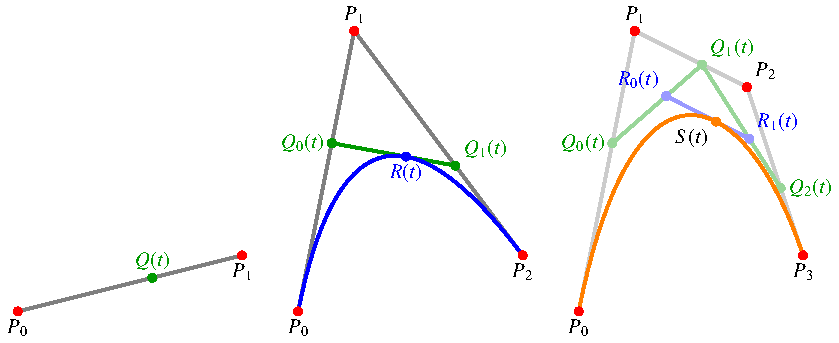
\includegraphics{chapters/30-interpolation/figures/bezier.pdf}
\caption{Bézier-Kurven bis zur Ordnung 3
\label{buch:interpolation:figure:bezier}}
\end{figure}
Die einfachste Verbindung zwischen zwei Punkten $P_0$ und $P_1$ mit
Ortsvektoren $p_0$ und $p_1$ ist eine Strecke, die man mit
\[
\gamma(t) = (1-t)p_0 + tp_1
\]
parametrisieren kann.
Der Tangentialvektor ist bereits bestimmt, er ist
\[
\dot{\gamma}(t) = -p_0 + p_1 = p_1-p_0.
\]
Die zwei Punkte legen den Tangentialvektor bereits fest, man kann
ihn nicht mehr frei wählen.

Kann man eine einfach zu berechnende Kurve finden, die den Punkt $P_0$
mit einem vorgegebenen Geschwindigkeitsvektor verlässt?
Paul de Casteljau hat vorgeschlagen, drei Punkte $P_0$, $P_1$ und $P_2$
zu verwenden und zunächst wie vorhin die Strecken 
\begin{align*}
q_0(t) &= (1-t) p_0 + t p_1 \\
q_1(t) &= (1-t) p_1 + t p_2 
\end{align*}
zu bilden.
Zur Zeit $t=0$ verlässt das erste Segment den Punkt $P_0$ mit der
Geschwindigkeit $p_1-p_0$.
Zur Zeit $t=1$ kommt das zweite Segment im Punkt $P_2$ an mit der
Geschwindigkeit $p_2-p_1$.
Man muss also zwischen $t=0$ und $t=1$ ``vom ersten Segment auf das zweite
wechseln''.
Dazu verbindet man die Punkte $q_0(t)$ und $q_1(t)$ mit einer Strecke und
wählt den Streckenparameter wieder als $t$.
Man erhält so eine Kurve
\begin{align*}
r(t)
&=
(1-t) q_0(t) + t q_1(t)
\\
&=
(1-t) \bigl( (1-t)p_0 + tp_1\bigr)
+
t \bigl( (1-t)p_1 + tp_2\bigr)
\\
&=
(1-t)^2 p_0 + 2t(1-t) p_1 + t^2 p_2.
\end{align*}
Der Geschwindigkeitsvektor zu den Zeiten $t=0$ und $t=1$ ist
\begin{align*}
\dot{r}(t)
&=
-2(1-t)p_0 + (2(1-t)-2t) p_1 + 2tp_2
\\
&=\begin{cases}
-2p_0+2p_1=2(p_1-p_0)&\qquad t=0
\\
-2p_1+2p_2=2(p_2-p_1)&\qquad t=1
\end{cases}
\end{align*}
Die gefundene Kurve verlässt also den Punkt $P_0$ genau in Richtung
auf $P_1$ und kommt im Punkt $P_2$ aus der Richtung von $P_1$ an.
Wir haben also eine quadratische Kurve gefunden, die einen Teil 
der Forderungen erfüllt.

Man nennt diese Kurve, dargestellt in
Abbildung~\ref{buch:interpolation:figure:bezier} Mitte,
eine quadratische {\em Bézier-Kurve} mit
\index{Bézier-Kurve}
{\em Kontrollpunkten} $P_0$, $P_1$ und $P_2$.
\index{Kontrollpunkte}
Der Punkt $P_1$ kontrolliert die Start- und Ankunftsrichtung.

\subsubsection{Kubische Bézier-Kurven}
Die beiden Richtungen in Anfangs- und Endpunkten müssen unabhängig
voneinander vorgegeben werden können, wir versuchen daher, die
gleiche Konstruktion mit vier Kontrollpunkten durchzuführen.
Gegeben seien jetzt also die Punkte $P_0,\dots,P_3$.
Dann können wir drei Strecken
\begin{align*}
q_0(t) &= (1-t) p_0 + t p_1 \\
q_1(t) &= (1-t) p_1 + t p_2 \\
q_2(t) &= (1-t) p_2 + t p_3 
\end{align*}
konstruieren.
Die erste hat die ``richtige'' Startrichtung, die letzte die ``richtige''
Ankunfsrichtung.
Kombinieren wir $q_0(t)$ und $q_1(t)$, erhalten wir eine quadratische
Kurve, die vom Punkt $P_0$ mit der richtigen Geschwindigkeit weggeht,
die Kombination von $q_1(t)$ mit $q_2(t)$ liefert eine quadratische
Bézier-Kurve, welche im Punkt $P_3$ mit der richtigen Geschwindigkeit
ankommt.
Wir können also erneut kombinieren:
\begin{equation}
\left.
\begin{aligned}
r_0(t) &= (1-t)q_0(t) + t q_1(t) \\
       &= (1-t)^2 p_0 + 2t(1-t) p_1 + t^2 p_2
\\
r_1(t) &= (1-t)q_1(t) + t q_2(t) \\
       &= (1-t)^2 p_1 + 2t(1-t) p_2 + t^2 p_3
\end{aligned}
\quad
\right\}
\quad\Rightarrow\quad
s(t) = (1-t) r_0(t) + t r_1(t)
\end{equation}
(siehe auch Abbildung~\ref{buch:interpolation:figure:bezier} rechts).
Wir berechnen 
\begin{equation*}
\begin{linsys}{5}
s(t) &=& (1-t) \bigl( (1-t)^2 p_0 &+& 2t(1-t)         p_1 &+& t^2     p_2 &\bigr) & \phantom{\bigr)}\\
     & &                          & & t\bigl( (1-t)^2 p_1 &+& 2t(1-t) p_2 &+& t^2p_3\bigr) \\
     &=& (1-t)^3 p_0 &+& 3t(1-t)^2 p_1 &+& 3t^2(1-t) p_2 &+& t^3 p_3\rlap{.}\phantom{\bigr)}
\end{linsys}
\end{equation*}
Der Tagententialvektor an den Stellen $t=0$ und $t=1$ ist
\begin{align*}
\dot{s}(t)
&=
-3(1-t)^2p_0 + (3(1-t)^2-6t(1-t))p_1 + (6t(1-t)-3t^2)p_2 + 3t^2p_3
\\
\Rightarrow\qquad
\dot{s}(0) &= -3p_0+3p_1 = 3(p_1-p_0)
\\
\dot{s}(1) &= -3p_2 + 3p_3 = 3(p_3-p_2),
\end{align*}
die Kurve verlässt also wie erwartet den Punkt $P_0$ genau in Richtung 
auf $P_1$ und kommt genau aus der Richtung von $P_2$ in $P_3$ an.

%
% Hermite-Interpolation
%
\subsubsection{Bézier-Kurven und Hermite-Interpolation}
\begin{figure}
\centering
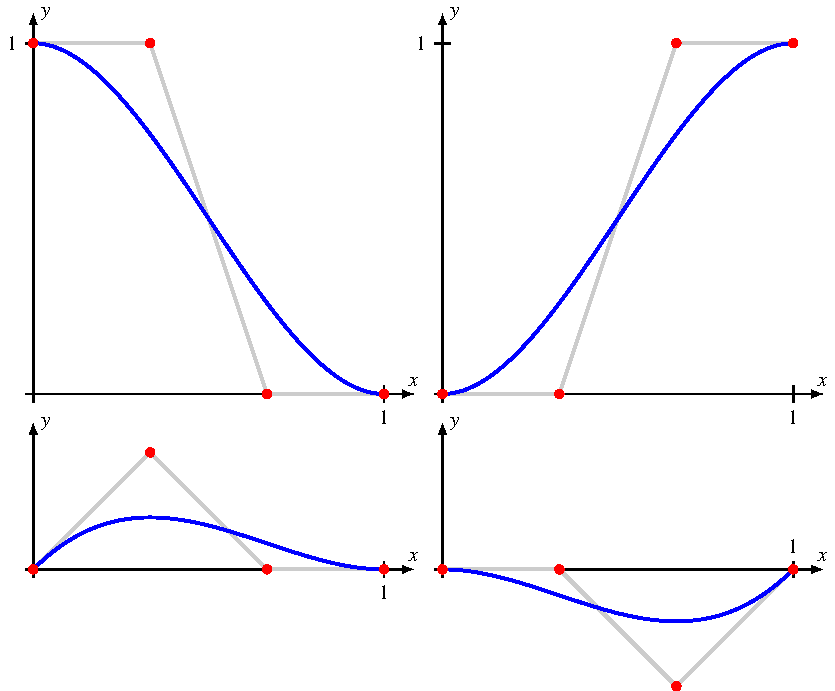
\includegraphics{chapters/30-interpolation/figures/bezierhermite.pdf}
\caption{Die Polynome $H_k(x)$ und $H_k^l(x)$ für $k=0,1$ und $l=0,1$
berechnet als Bézier-Kurven der Ordnung 3.
\label{buch:bezier:figure:bezierhermite}}
\end{figure}
Man kann auch die Spline-Funktionen wieder aus der zweidimensionalen
Kurve $s(t)$ rekonstruieren.
Gegeben sind dafür zwei Werte $y_0$ und $y_1$ und die Steigungen $m_0$ und
$m_1$ in den Punkten $x=0$ und $x=1$.
Der Graph des kubischen Polynoms $p(x)$ mit $p(0)=y_0$, $p(1)=y_1$,
$p'(0)=m_0$ und $p'(1)=m_1$ soll jetzt als Bézier-Kurve geschrieben werden.
Dazu müssen die Kontrollpunkte gefunden werden.
Es ist klar, dass $P_0=(0,y_0)$ und $P_3=(1,y_1)$.
Für die inneren Kontrollpunkte muss ein geeigneter $x$-Wert gewählt werden,
also
\[
P_1=
(x_1,y_0+x_1m_0)
\qquad
\text{und}
\qquad
P_2
=
(x_2,y_1-(1-x_2)m_1)
\]
Wählt man $x_1=\frac13$ und $x_2=\frac23$, dann wird
\begin{align*}
x(t)
&=
(1-t)^3\cdot 0 + 3t(1-t)^2\cdot \frac13 + 3t^2(1-t)\cdot \frac23 + t^3\cdot 1
\\
&=
t-2t^2+t^3 + 2t^2 -2t^3 + t^3 = t.
\end{align*}
Mit dieser Wahl ist also $x=t$, so dass das gesuchte Polynom $p(x)=y(x)$ wird:
\begin{align*}
p(x)
=
y(x)
&=
(1-x)^3 y_0
+
3x(1-x)^2\biggl(y_0+\frac13m_0\biggr)
+
3x^2(1-x) \biggl(y_1-\frac13m_1\biggr)
+
x^3 y_1
\\
&=
\bigl((1-x)^3+3x(1-x)^2\bigr)
y_0
+
x(1-x)^2 m_0
-
x^2(1-x) m_1
+
\bigl(3x^2(1-x)+x^3\bigr)
y_1
\\
&=
(1+2x)(1-x)^2 y_0
+
x(1-x)^2 m_0
+
x^2(x-1) m_1
+
x^2(3-2x) y_1.
\end{align*}
Die Koeffizienten von $y_0$, $y_1$, $m_0$ und $m_1$ sind die Polynome
\begin{equation}
\begin{aligned}
y_0:&&
H_0(x)
&=
2x^3-3x^2+1
&\quad&
&m_0:&&
H_0^1(x)
&=
x-2x^2+x^3
\\
y_1:&&
H_1(x)
&=
3x^2-2x^3
&\quad&
&m_1:&&
H_1^1(x)
&=
x^3-x^2
\end{aligned}
\label{buch:bezier:eqn:H}
\end{equation}
Die Polynome \eqref{buch:bezier:eqn:H} stimmen mit den Polynomen überein,
die in \eqref{buch:equation:hermite:h} gefunden worden sind.

%
% Bézier-Kurven höherer Ordnung
%
\subsubsection{Bézier-Kurven höherer Ordnung}
Der Prozess, der die kubischen Bézier-Kurven produziert hat, kann natürlich
iteriert werden, um Kurven beliebiger Ordnung zu erzeugen.
Ausgehend von $n+1$ Kontrollpunkten $P_0,\dots,P_n$, konstruiert man eine
rekursiv eine Folge von Punkten wie folgt.
Zunächst setzt man $P_{0k}(t) = P_k$ mit zugehörigen Ortsvektoren $p_{0k}(t)$.
Dann definiert man die {\em konvexe Kombination} der beiden Kurven als
\begin{align*}
p_{ik}(t) &= (1-t)  p_{i-1,k}(t) + p_{i-1,k+1}(t)
\qquad
1\le i \le n,\; 
0\le k\le n - i.
\end{align*}
Der Vektor $p_{n0}(t)$ beschreibt eine Kurve vom Grad $n-1$.
\begin{figure}
\centering
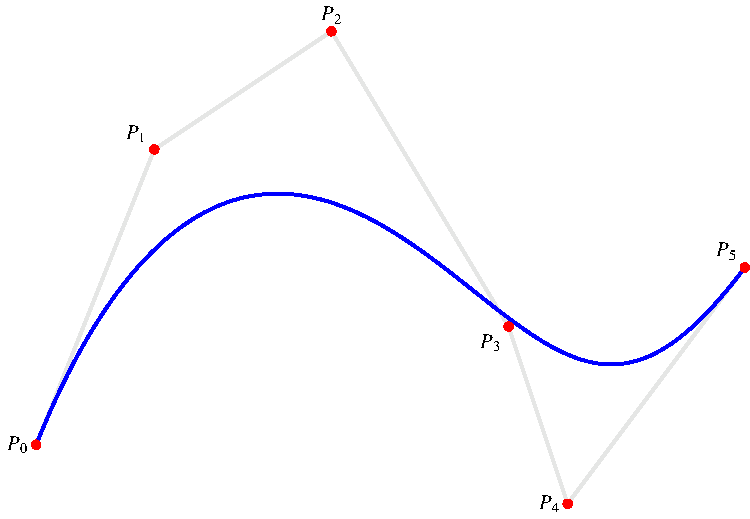
\includegraphics{chapters/30-interpolation/figures/beziern.pdf}
\caption{Bézier-Kurve vom Grad 5 mit 6 Kontrollpunkten.
\label{buch:bezier:figure:beziern}}
\end{figure}
In Abbildung~\ref{buch:bezier:figure:beziern} ist eine Bézier-Kurve
der Ordnung $5$ mit 6 Kontrollpunkten dargestellt.

\begin{figure}
\centering
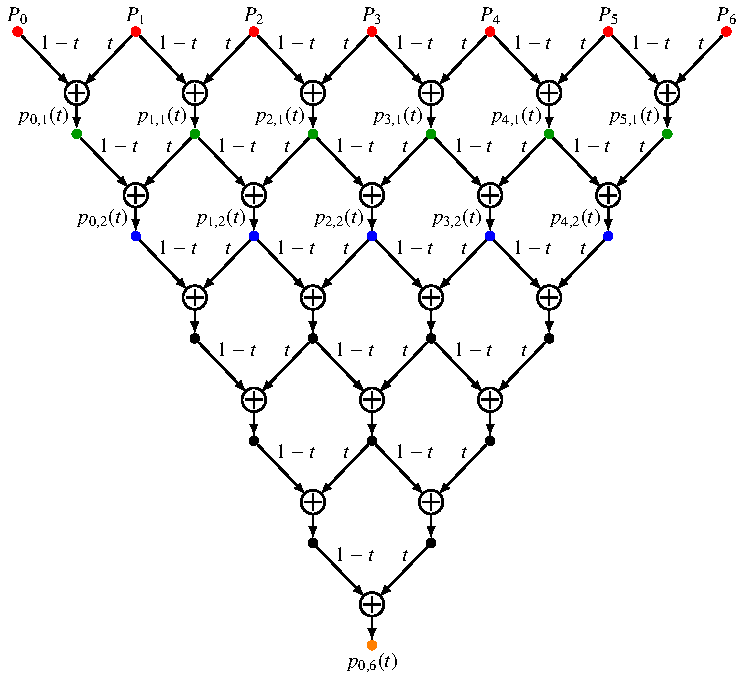
\includegraphics{chapters/30-interpolation/figures/bezierberechnung.tex}
\caption{Berechnungsschema für die Koordinaten eines Punktes einer Bézier-Kurve
mit $7$ Kontrollpunkten.
Jeder schräge Pfeil entspricht zwei Multiplikationen.
Die Anzahl Multiplikationen ist viermal so gross wie die Zahl der Summationen.
\label{buch:bezier:figure:bezierberechnung}}
\end{figure}
Der rekursive Berechnungsprozess von $p_{n0}(t)$ ist in
Abbildung~\ref{buch:bezier:figure:bezierberechnung} schematisch
dargestellt.
Jeder schräge Pfeil steht für zwei Multiplikationen,
für jeden Summenknoten sind also vier Multiplikationen und zwei Additionen
auszuführen.
Daraus kann man ablesen, dass die Berechnung von $s(t)$ genau
\begin{align}
4\cdot (1 + 2 + \dots + n) &= 4\sum_{k=1}^n k = 2n(n+1)
\label{buch:bezier:eqn:multiplikationen}
\end{align}
Multiplikationen und $n(n+1)$ Additionen benötigt.

\begin{satz}
\label{buch:bezier:satz}
Die Kurve $p_{n0}(t)$ hat die Eigenschaft
\begin{align*}
\dot{p}_{n0}(0) &= n (p_1-p_0)
\\
\dot{p}_{n0}(1) &= n (p_n-p_{n-1}).
\end{align*}
In expliziter Form gilt
\[
p_{n0}(t)
=
\sum_{k=0}^n \binom{n}{k} t^k(1-t)^{n-k} p_k
=
\sum_{k=0}^n B_{k,n}(t) p_k
\]
wobei $B_{k,n}(t) = \binom{n}{k}t^k(1-t)^{n-k}$
die sogenannten {\em Bernsteinpolynome} sind.
\end{satz}

Man braucht immer die Werte aller Bernsteinpolynome.
Dazu berechnet man in $2(n-1)$ Multiplikationen zuerst alle
Potenzen von $t$ und $(1-t)$.
Mit $2(n-1)$ weiteren Multiplikationen bekommt man dann die Werte
der Bernsteinpolynome.
Insgesamt sind also $4(n-1)$ Multiplikationen für die Bernstein-Polynome
nötig.
Die Berechnung der Bézier-Kurve benötigt nochmals $2(n+1)$ Multiplikationen
und $2n$ Additionen.
Insgesamt sind also $6n-2$ Multiplikationen und $2n$ Addition nötig.
Die Berechnung nach dem Schema von 
Abbildung~\ref{buch:bezier:figure:bezierberechnung} wächst dagegen 
quadratisch mit $n$ an.
Für $n\ge 2$ folgt aus \eqref{buch:bezier:eqn:multiplikationen}
dass das rekursive Verfahren mindestens $2n\cdot 3=6n$ und damit
bereits mehr Multiplikationen benötigen.

\begin{proof}[Beweis]
Die Terme mit $p_k$ im Polynom $p_{0n}(t)$ kann man aus
Abbildung~\ref{buch:bezier:figure:bezierberechnung} ablesen.
Jeder Weg von $p_k$ zum Polynom $p_{0n}(t)$ setzt sich zusammen aus
einer $k$ Links-Pfeilen und $n-k$ Rechts-Pfeilen.
Jeder Weg trägt daher einen Summanden $t^k(1-t)^{n-k}$ bei.
Wie beim Pascal-Dreieck kann man einsehen, dass es $\binom{n}{k}$
solche Wege gibt.
Damit ist die Formel für die Koeffizienten beweisen.
Durch Ableiten könnte man auch die Behauptung über den Tangentialvektor
am Anfang und am Ende der Kurve beweisen.
\end{proof}

Die Eigenschaften des Tagentialvektors bei $t=0$ und $t=1$
der Kurve $p_{0n}(t)$ lässt sich aber mit Hilfe der Rekursionsformel
auch direkt nachweisen.

\begin{lemma}
Sind $p(t)$ und $q(t)$ zwei beliebige Kurven derart, dass
$\dot{p}(0) = \alpha( q(0)-p(0))$ und $\dot{q}(1) \beta( q(1)-p(1))$,
dann ist
$\gamma(t) = (1-t)p(t) + tq(t)$
eine Kurve mit
$\dot{\gamma}(0)=(\alpha+1)(q(0)-p(0))$
und
$\dot{\gamma}(1)=(\beta+1)(q(1)-p(1))$.
\end{lemma}

\begin{proof}[Beweis]
Wir berechnen die Ableitung von $\gamma(t)$
\begin{align*}
\dot{\gamma}(t)
&=
-p(t) + (1-t)\dot{p}(t) + q(t) + t\dot{q}(t)
\\
\dot{\gamma}(0)
&=
-p(0) + q(0) + \dot{p}(0)
=
(1+\alpha)(q(0)-p(0)),
\\
\dot{\gamma}(1)&=-p(1) + q(1) + \dot{q}(1)
=
(1+\beta)(q(1)-p(1)).
\qedhere
\end{align*}
\end{proof}

Wir können jetzt den Beweis der Eigenschaften des Tangentialvektors
mit Hilfe von vollständiger Induktion abschliessen.
Die Polynome $p_{k0}(t)$ haben die im Lemma formulierte Eigenschaft,
denn es ist
$\dot{p}_{k0}(t) = 0$
und daher
\begin{align*}
\dot{p}_{k0}(0)
&=
0\cdot p_{k+1,0}(0) - p_{k,0}(0) = 0\cdot(p_{k+1}-p_{k})
\\
\dot{p}_{k0}(1)
&=
0\cdot p_{k+1,0}(1) - p_{k,0}(1) = 0\cdot(p_{k+1}-p_{k}).
\end{align*}
Nehmen wir jetzt an, die Eigenschaft sei für Bézier-Kurven vom Grad $l$
bereits beweisen.
Die Kurve $p_{kl}(t)$ ist eine Bézier-Kurve mit den Kontrollpunkten
$P_k,\dots,P_{k+l}$.
Dies bedeutet, dass die Kurven $p_{kl}(t)$ den Tangentialvektor
\begin{align*}
\dot{p}_{kl}(0)&= l(p_{k}-p_{k+1}) \\
\dot{p}_{kl}(1)&= l(p_{k+l}-p_{k+l-1})
\end{align*}
haben.
Ausserdem ist $p_{kl}(0) = p_k$ und $p_{kl}(1) = p_{k+l}$, so dass auch
die Bedingung über die Endpunkte im Lemma erfüllt ist.
Es folgt daher mit Hilfe des Lemmas für die konvexe Kombination $p_{k,l+1}(t)$
von $p_{kl}(t)$ und $p_{k+1,l}(t)$
\begin{align*}
\dot{p}_{k,l+1}(0)
&=
(1+l)(p_{k,l+1}(0) - p_{k,l}(0))
=
(l+1)(p_{k+1} - p_{k})
\\
\dot{p}_{k,l+1}(1)
&=
(1+l)(p_{k,l+1}(1) - p_{k,l}(1))
=
(l+1)(p_{k+l+1}-p_{k+l}).
\end{align*}
Damit ist der Induktionsschritt vollzogen und alles bewiesen.

